%%%%%%%%%%%%%%%%%%%%%%%%%
% Dokumentinformationen %
%%%%%%%%%%%%%%%%%%%%%%%%%
\newcommand{\titleinfo}{Wahrscheinlichkeitsrechnung und Statistik - Formelsammlung}
\newcommand{\authorinfo}{Braun \& Co, J.Rast}
\newcommand{\versioninfo}{$Revision: 1 $ - powered by \LaTeX} 

%%%%%%%%%%%%%%%%%%%%%%%%%%%%%%%%%%%%%%%%%%%%%
% Standard projektübergreifender Header für
% - Makros 
% - Farben
% - Mathematische Operatoren
%
% DORT NUR ERGÄNZEN, NICHTS LÖSCHEN\newpage
%%%%%%%%%%%%%%%%%%%%%%%%%%%%%%%%%%%%%%%%%%%%%
% Genereller Header
\documentclass[10pt,a4paper,fleqn]{article}
% Dateiencoding
\usepackage[utf8]{inputenc}
% Seitenränder
\usepackage[left=2cm,right=2cm,top=1cm,bottom=1cm,includeheadfoot]{geometry}
% Sprachpaket
\usepackage[ngerman]{babel,varioref}

% Pakete
\usepackage{amssymb,amsmath,fancybox,graphicx,color,lastpage,wrapfig,fancyhdr,hyperref,verbatim,floatflt,multicol,multirow,rotating,pdflscape,array,longtable,listings}

% Zum Bilder einfach in Tabellen einfügen (valign=t)
\usepackage[export]{adjustbox}

%%%%%%%%%%%%%%%%%%%%
% Generelle Makros %
%%%%%%%%%%%%%%%%%%%%
\newcommand{\skript}[1]{$_{\textcolor{red}{\mbox{\small{Skript S.#1}}}}$}
\newcommand{\verweis}[2]{\small{(siehe auch \ref{#1}, #2 (S. \pageref{#1}))}}
\newcommand{\verweiskurz}[1]{(\small{siehe \ref{#1}\normalsize)}}
\newcommand{\subsubadd}[1]{\textcolor{black}{\mbox{#1}}}
\newcommand{\formelbuch}[1]{$_{\textcolor{red}{\mbox{\small{S#1}}}}$}

\newcommand{\kuchling}[1]{$_{\textcolor{red}{\mbox{\small{Kuchling #1}}}}$}
\newcommand{\stoecker}[1]{$_{\textcolor{grey}{\mbox{\small{Stöcker #1}}}}$}
\newcommand{\sachs}[1]{$_{\textcolor{blue}{\mbox{\small{Sachs S. #1}}}}$}
\newcommand{\hartl}[1]{$_{\textcolor{green}{\mbox{\small{Hartl S. #1}}}}$}


\newcommand{\skriptsection}[2]{\section{#1 {\tiny Skript S. #2}}}
\newcommand{\skriptsubsection}[2]{\subsection{#1 {\tiny Skript S. #2}}}
\newcommand{\skriptsubsubsection}[2]{\subsubsection{#1 {\tiny Skript S. #2}}}

\newcommand{\matlab}[1]{\footnotesize{(Matlab: \texttt{#1})}\normalsize{}}

%%%%%%%%%%
% Farben %
%%%%%%%%%%
\definecolor{black}{rgb}{0,0,0}
\definecolor{red}{rgb}{1,0,0}
\definecolor{white}{rgb}{1,1,1}
\definecolor{grey}{rgb}{0.8,0.8,0.8}
\definecolor{green}{rgb}{0,.8,0.05}
\definecolor{brown}{rgb}{0.603,0,0}

%%%%%%%%%%%%%%%%%%%%%%%%%%%%
% Mathematische Operatoren %
%%%%%%%%%%%%%%%%%%%%%%%%%%%%
\DeclareMathOperator{\sinc}{sinc}
\DeclareMathOperator{\sgn}{sgn}
\DeclareMathOperator{\Real}{Re}
\DeclareMathOperator{\Imag}{Im}
\DeclareMathOperator{\e}{e}
\DeclareMathOperator{\cov}{cov}
\DeclareMathOperator{\PolyGrad}{PolyGrad}


%%%%%%%%%%%%%%%%%%%%%%%%%%%
% Fouriertransformationen %
%%%%%%%%%%%%%%%%%%%%%%%%%%%
\unitlength1cm
% Zeitbereich -- Frequenzbereich
\newcommand{\laplace}
{
\begin{picture}(1,0.5)
\put(0.2,0.1){\circle{0.14}}\put(0.27,0.1){\line(1,0){0.5}}\put(0.77,0.1){\circle*{0.14}}
\end{picture}
}
% Frequenzbereich -- Zeitbereich
\newcommand{\Laplace}
{
\begin{picture}(1,0.5)
\put(0.2,0.1){\circle*{0.14}}\put(0.27,0.1){\line(1,0){0.45}}\put(0.77,0.1){\circle{0.14}}
\end{picture}
}

% Fouriertransformationen
\unitlength1cm
\newcommand{\FT}
{
\begin{picture}(1,0.5)
\put(0.2,0.1){\circle{0.14}}\put(0.27,0.1){\line(1,0){0.5}}\put(0.77,0.1){\circle*{0.14}}
\end{picture}
}


\newcommand{\IFT}
{
\begin{picture}(1,0.5)
\put(0.2,0.1){\circle*{0.14}}\put(0.27,0.1){\line(1,0){0.45}}\put(0.77,0.1){\circle{0.14}}
\end{picture}
}




%%%%%%%%%%%%%%%%%%%%%%%%%%%%
% Allgemeine Einstellungen %
%%%%%%%%%%%%%%%%%%%%%%%%%%%%
%PDF Info
\hypersetup{pdfauthor={\authorinfo},pdftitle={\titleinfo},colorlinks=false}
\author{\authorinfo}
\title{\titleinfo}

%%%%%%%%%%%%%%%%%%%%%%%
% Kopf- und Fusszeile %
%%%%%%%%%%%%%%%%%%%%%%%
\pagestyle{fancy}
\fancyhf{}
%Linien oben und unten
\renewcommand{\headrulewidth}{0.5pt} 
\renewcommand{\footrulewidth}{0pt}

\fancyhead[L]{\titleinfo{ }}
%Kopfzeile rechts bzw. aussen

%Fusszeile links bzw. innen

%Fusszeile rechts bzw. ausen

% Einrücken verhindern versuchen
\setlength{\parindent}{0pt}

% Zeilenhöhe Tabellen:
\newcommand{\arraystretchOriginal}{1.5}
\renewcommand{\arraystretch}{\arraystretchOriginal}



% Möglichst keine Ergänzungen hier, sondern in header.tex
\begin{document}

\setlength{\parindent}{0pt}
%%%%%%%%%%%%%%%%%%%%%%%%%%%%%%%%%%%%%%%%%%%%%%%%%%%%%%%%%%%%%%%%%%%%%%%%%%%%%%%%%%%%%%%%%%%%%%%%
%%%%%%%%%%%%%%%%%%%%%%%%%%%%%%%%%%%%%%%%%%%%%%%%%%%%%%%%%%%%%%%%%%%%%%%%%%%%%%%%%%%%%%%%%%%%%%%%
\section{Ereignisse und ihre Wahrscheinlichkeit}
%\renewcommand{\baselinestretch}{1.25}\normalsize
	\subsection{Kombinatorik \sachs{66}}
		\begin{minipage}{13.5cm}
		\begin{tabular}{| p{5.5cm} | c | c |}
			\hline
			Art der Auswahl bzw. Zusammenstellung von $k$ aus $n$ Elementen
			& \multicolumn{2}{c|}{Anzahl der Möglichkeiten}\\
 			& ohne Wiederholungen		& mit Wiederholungen\\
 			& $(k\leq n)$ 				& $(k\leq n)$ \\
 			\hline
 			Permutationen & $P_n=n!(n=k)$ &
 			$P_n^{(k)}=\frac{n!}{k!}$ \\ & &\\
 			Kombinationen & $C_n^{(k)}=\binom n k$ &
 			$C_n^{(k)}=\binom{n+k-1} k$\\
 			& &\\
 			Variationen & $V_n^{(k)}=k!\binom n k$ & $V_n^{(k)}=n^k$\\
 			\hline
		\end{tabular}
		\end{minipage}
		\begin{minipage}{5cm}
		$\binom n k$ mit TR: \texttt{nCr(n,k)} \hspace{9.3mm}En\\
		\hspace*{19mm} \texttt{Kombinat(n,k)} De
		\end{minipage}
		\begin{list}{$\bullet$}{\setlength{\itemsep}{0cm} \setlength{\parsep}{0cm} \setlength{\topsep}{0.1cm}} 
         	\item \textbf{Permutationen}: Gegeben seien $n$ verschiedene Objekte. Dann gibt es $n!$
         	verschiedene Reihenfolgen in denen man diese Objekte anordnen
         	kann. \\
         	z.B.: $x,y,z;\quad x,z,y;\quad z,y,x;\ldots$
         % \item Permutation nennt man eine Anordnung von $n$ Elementen in einer Bestimmten
		%		Reihenfolge
		 	\item \textbf{Kombination}: Gegeben seien $n$ verschiedene Objekte. Dann gibt es $\binom n k$
		 	Möglichkeiten, daraus $k$ Objekte auszuwählen, wenn es nicht auf die Reihenfolge
		 	ankommt. \\
		 	z.B.: Wie viele verschiedene Möglichkeiten hat man beim Lotto, 6 Zahlen aus 49
		 	auszuwählen?
		 % \item Kombination nennt man eine Auswahl von $k$ Elementen aus $n$ Elementen
		 % 		ohne Beachtung der Reihenfolge
		  \item \textbf{Variation} nennt man eine Auswahl von $k$ Elementen aus $n$
		  		verschiedenen Elementen unter Beachtung der Reihenfolge
        \end{list}
        
\hrule
\vspace{5mm}
	\begin{minipage}{6.8cm}
	\subsection{Wahrscheinlichkeit\skript{18}}
		\begin{tabular}{ll}
			Wertebereich:
			& ${0}\le{P(A)}\le{1}$\\ \\
			Sicheres Ereignis:
			& $P(\Omega)=1$\\ \\
			unmögliches Ereignis:
			& $P(\emptyset)=0$
		\end{tabular}
	\end{minipage}
		\begin{minipage}{11.2cm}
		\subsubsection{Rechenregeln}
			\begin{tabular}{ll}
				komplementär Ereignis:
				&$P(\bar{A})=P({\Omega}\setminus{A})=1-P(A)$\\ \\
				Differenz der Ereignisse A und B:
				&$P({A}\setminus{B})=P(A)-P({A}\cap{B})$\\ \\
				Vereinigung zweier Ereignisse:
				&$P({A}\cup{B})=P(A)+P(B)-P({A}\cap{B})$
			\end{tabular}
		\end{minipage}
\vspace{1mm}
\hrule
	
	\subsection{Laplace-Ereignisse \skript{37} \sachs{79}}
    	In einem endlichen Wahrscheinlichkeitsraum $\Omega$ haben alle
    	Elementarereignisse die gleiche Wahrscheinlichkeit.
    	\begin{center}
    	$P(A)=\dfrac{\left| A\right|}{\left|\Omega\right|}$
    	\end{center}


\hrule

	\subsection{Unabhängige Ereignise \skript{24} \sachs{83}}
		Unabhängige Ereignisse $A$ und $B$ liegen vor, wenn:\\
    	\hspace*{8mm} $P(A\mid B)=P(A)$ \hspace{4mm} und \hspace{4mm}
    	$P(B\mid A)=P(B)$\\
    	erfüllt ist. Für sie gilt\\
    	\hspace*{8mm} $P(A\cap B)=P(A)P(B)$\\
    	Die Tatsache, dass A eingetreten ist, hat keinen Einfluss auf die 
		Wahrscheinlichkeit von B.\vspace{1mm}

\hrule

	\subsection{Bedingte Wahrscheinlichkeit \skript{26} \sachs{85}}
		Die Wahrscheinlichkeit für das Eintreten des Ereignisses $A$ unter der
		Bedingung, dass das Ereignis $B$ bereits eingetreten ist.
		\begin{center}
		$P(A\mid B)= \dfrac{P(A\cap B)}{P(B)}=\underbrace{\frac{P(A)\cdot
		P(B)}{P(B)}=P(A)}_{\text{nur wenn unabhängig}}$ 
		\end{center}

\hrule

	\subsection{Satz von Bayes \skript{30} \sachs{89}}
		\begin{tabular}{ll}
		$P(B\mid A)=P(A\mid B) \cdot\dfrac{P(B)}{P(A)}$\vspace{1mm}
		\end{tabular}

\hrule
	\subsection{Totale Wahrscheinlichkeit \skript{29} \sachs{88}}
		\begin{tabular}{ll}
        $P(A)=\sum\limits_{i=1}^N P(A\mid G_i)\cdot P(G_i)$
        \end{tabular}

\newpage
\section{Erwartungswert und Varianz}

	\subsection{Erwartungswert \skript{55} \sachs{101}}
		Sei $X$ eine Funktion auf $\Omega$, und lasse sich $\Omega$ in endlich viele
		Ereignisse, auf denen $X(\omega)$ konstant ist, $A_i$ zerlegen, dann ist der
		Erwartungswert von $X$\\
        \hspace*{5.7cm}$Erwartungswert = \sum Wert \cdot Wahrscheinlichkeit$\\
		\hspace*{7.5cm}$E(X)=\sum\limits_{i=0}^n
		\underbrace{X(A_i)}_{\text{Wert}}\cdot \underbrace{P(A_i)}_{\text{W'keit}}$\\
		\hspace*{5.7cm}$E(X) = \int\limits_{-\infty}^x x \cdot \varphi(x) dx$ mit
		$\varphi(x) = Dichtefunktion$ 

		\subsubsection{Rechenregeln}
			\begin{tabular}{ll}
    		$E(X+Y)=E(X)+E(Y)$\\
    		$E(\lambda X + \mu)=\lambda \cdot E(X) + \mu$ & $\lambda, \mu \in \mathbb{R}$\\
    		$E(XY) = E(X)\cdot E(Y)$ & wenn X,Y unabhängig sind\\
    		\end{tabular}

\vspace{1mm}
\hrule
\vspace{2mm}

	\begin{minipage}{9cm}
	\subsection{Varianz \skript{63} \sachs{106}}
		\begin{tabular}{ll}
		$var(x)=\sigma ^2=E[(X-E(X))^2]=E(X^2)-E(X)^2$\\
		\end{tabular}

		\subsubsection{Kovarianz \sachs{49}}
		\begin{tabular}{ll}
        $cov(X,Y)=E(XY)-E(X)E(Y)=\underbrace{0}_{\text{falls X,Y unabhängig}}$
        \end{tabular}
	\end{minipage}
		\begin{minipage}{9cm}
		\subsubsection{Rechenregeln}
			\begin{tabular}{ll}
        	$var(\lambda X)=\lambda^2 var(X) \qquad $ $\lambda, \mu \in
        	\mathbb{R}$\\ 
        	$var(X_1+X_2+\ldots+X_n) \neq var(n X)$ \\
        	$var(X+Y)= \begin{cases}
	                      var(X)+var(Y)
	                      &	\text{(X,Y unabh.)}\\                     
	                      var(X) + var(Y) + 2 \cdot cov(X,Y) 
	                      &	\text{(X,Y abhängig)}\\
                     \end{cases} $ \\
        	$var(X Y)= var(Y)var(X)+var(Y)E(X)^2+var(X)E(Y)^2$
        	\end{tabular}
		\end{minipage}
\vspace{1mm}

\hrule

		\subsection{Erwartungswert und Varianz des arithmetischen Mittels \skript{68}}
		Es sei eine folge von unabhängigen Zufallsvariablen $X_1, X_2, \ldots , X_n$ mit gleichem
		Erwartungswert $ \mu $ und gleicher Varianz $ \sigma^2 $ gegeben.  \\
		\begin{tabular}{p{6cm} p{6cm} p{6cm}}
	        Mittelwert: $M_n=\frac{X_1+\ldots+X_n}{n}$ 
	        & Erwartungswert: $E(X)=E(M_n)$
	        & Varianz: $var(M_n)=\frac{1}{n}var(X)$
        \end{tabular}
\vspace{1mm}

\hrule

\vspace{2mm}
	\begin{minipage}[]{9cm}
	\subsection{Regression \skript{70} \sachs{60, 141}}
		\begin{tabular}{ll}
        Allgemein: & X,Y Zufallsvariable\\
        Gesucht: & Regressionsgerade $y=ax+b$ mit min. Fehler\\
        Fehler: & $E(Y-(aX+b))=0$
        \end{tabular}
		\vspace{.1cm}

		\textbf{Regressionskoeffizient r}\\
        r ist ein Mass für die Qualität der Regression (standardisiert)\\
        $r^2=\dfrac{cov(X,Y)^2}{var(X)var(Y)}$ \\
        
		\textbf{Mittlerer quadratischer Fehler}\\
        $ \Delta^2 = var(Y)(1-r^2) =
        var(Y)\left(1-\dfrac{cov(X,Y)^2}{var(X)var(Y)}\right) $ \\
        
        \textbf{Berechnung mit Taschenrechner (TI-89, V-200)}
        \begin{list}{$\bullet$}{\setlength{\itemsep}{0cm}
        \setlength{\parsep}{0cm} \setlength{\topsep}{0cm}}  
	        \item Vorbereitung:\\
	        \texttt{$\{x_1, \ldots, x_n\} \blacktriangleright$\texttt{l1}$; \; 
	        \{y_1, \ldots,y_n\}\blacktriangleright$ \texttt{l2}$; \;$} \texttt{LinReg l1,l2}
	        \item Anzeige von Werten mit \\ \texttt{ShowStat}
	        \item Anzeige des Graphs mit \\
	        \texttt{reqeq(x)}$\blacktriangleright$\texttt{y1(x)}$; \;$
	        \texttt{NewPlot 1,1,l1,l2}
        \end{list}
	\end{minipage}
	\begin{minipage}{10cm}
    
	\textbf{Vorgehen:} \textcolor{grey}{mit Fehlerberechnung}
	\begin{enumerate}
		\item Tabelle mit bekannten Werten aufstellen:\\
		\begin{tabular}{|l||l|l||l|l||l|}
		\hline
		\textbf{$k$} & \textbf{$x$} & \textbf{$x^2$} & \textbf{$y$} &
		\textcolor{grey}{\textbf{$y^2$}} & \textbf{$xy$} \\ \hline \hline
		$1$ & $x_1$ & $x_1^2$ & $y_1$ & \textcolor{grey}{$y_1^2$} & $x_1y_1$ \\ \hline
		$\vdots$ & $\vdots$ & $\vdots$ & $\vdots$ & \textcolor{grey}{$\vdots$} &
		$\vdots$ \\\hline
		$n$ & $x_n$ & $y_n^2$ & $y_n$ & \textcolor{grey}{$y_n^2$} & $x_ny_n$ \\ \hline
		\hline
		$\sum$ & $\sum x_k$ & $\sum x_k^2$ & $\sum y_k$ & \textcolor{grey}{$\sum
		y_k^2$} & $\sum x_ky_k$ \\ \hline
		$E$ & $\frac{\sum x_k}{n}$ & $\frac{\sum x_k^2}{n}$ & $\frac{\sum y_k}{n}$ &
		\textcolor{grey}{$\frac{\sum y_k^2}{n}$} & $\frac{\sum x_ky_k}{n}$ \\ \hline
		\end{tabular} 

		\item Varianzen, Kovarianz berechnen:\\
		$var(X) = E(X^2) - E^2(X)$ \\
		\textcolor{grey}{$var(Y) = E(Y^2) - E^2(Y)$} \\
		$cov(X,Y) = E(XY) - E(X)E(Y)$
		\item Koeffizienten \textcolor{grey}{und Fehler} der Gerade berechnen:\\
		$a=\dfrac{cov(X,Y)}{var(X)}$
		\textcolor{grey}{$\qquad\Delta^2=var(Y)\left(1-\dfrac{cov(X,Y)^2}
		{var(X)var(Y)}\right) $}\\ $b=E(Y)-aE(X)$
		\item Gerade:\\
		$y=ax+b$
	\end{enumerate}
	\end{minipage}
\vspace{2mm}
\hrule
		
	\subsection{Satz von Tschebyscheff \skript{67}}
		\begin{tabular}{ll}
        $P(\left| X-E(X)
        \right|>\varepsilon)\leq\dfrac{var(X)}{\varepsilon^2}$ &
        Wahrscheinlichkeit, dass $X$ um mehr als $\varepsilon$ vom
        Erwartungswert $E(X)$ abweicht.\\
        $P(|M_{n}-\mu|>\varepsilon)\leq \frac{\sigma^{2}}{\varepsilon^{2}n} $ &
        W'keit, dass $M_{n}$ von $n$ unab. ZV mit Mittelwert $\mu$ und
        Varianz $\sigma^{2}$ mehr als $\varepsilon$ von $\mu$ abweicht.
        \end{tabular}

\newpage

\section{Wahrscheinlichkeitsverteilung}

	\subsection{Verteilungsfunktion \skript{77} \sachs{93 (diskret), 97
	(kontinuierlich)}}
		\renewcommand{\arraystretch}{1.5}
		\begin{tabular}[]{|l|l|}
        	\hline
        	\textbf{diskret} & \textbf{kontinuierlich}\\
        	\hline
        	\hline
        	$P(X\leq x)=F(x)=\sum\limits_{k=-\infty}^x p_k$ &
        	$P(X\leq x)=F(x)=\int\limits_{-\infty}^x
        	\varphi(\tilde{x})d\tilde{x}$\\
  			$P(X>x)=1-P(X\leq x)$ & $P(X>x)=1-P(X\leq x)$\\        	
        	$P(a \le X \leq b)=F(b)-F(a)=\sum\limits_{k=a}^b p_k$ &
  			$P(a \le X \leq b)=F(b)-F(a)=\int \limits_a^b
  			\varphi(\tilde{x})d\tilde{x}$\\
        	\hline
        \end{tabular}
		\renewcommand{\arraystretch}{1}

		\subsubsection{Eigenschaften}
  				$$\boxed{\mathbb{D}(F) = \mathbb{R}} \qquad \boxed{\mathbb{W}(F)
  				\in[0,1]} \qquad \boxed{F(-\infty)=0} \qquad  \boxed{F(\infty)=1}
  				\qquad \boxed{F(x) \text{ ist monoton steigend}}$$

\hrule

\vspace{5mm}
	\begin{minipage}{13cm}
	\subsection{Wahrscheinlichkeitsdichte \sachs{97}}
		\begin{tabular}{p{3.3cm}p{8.5cm}}
    	$\varphi(x)=F'(x)$ &Dichtefunktion oder Wahrscheinlichkeitsdichte\\
    	\multirow{2}{11cm}{Bei Sprungstellen von F(x): }\\
    	\multirow{2}{11cm}{$\varphi(x) = $ Dirac mit Gewichtung der Sprunghöhe}
    	
    	\end{tabular}
	\end{minipage}
	\begin{minipage}{5cm}
		\subsubsection{Erwartungswert}
			\begin{tabular}{ll}
            $\textcolor{red}{E(}\textcolor{green}{X}\textcolor{red}{)}=
        	\textcolor{red}{\int} \textcolor{green}{x} \cdot 
        	\textcolor{red}{\varphi(x)dx}$\\
        	$\textcolor{red}{E(}\textcolor{green}{X^2}\textcolor{red}{)}=
        	\textcolor{red}{\int} \textcolor{green}{x^2} \cdot 
        	\textcolor{red}{\varphi(x)dx}$\\ 
        	$\textcolor{red}{E(}\textcolor{green}{X^N}\textcolor{red}{)}=
        	\textcolor{red}{\int} \textcolor{green}{x^N} \cdot 
        	\textcolor{red}{\varphi(x)dx}$\\ 
%         	$\textcolor{red}{E(}\textcolor{green}{\sin X}\textcolor{red}{)}=
%         	\textcolor{red}{\int} \textcolor{green}{\sin x} \cdot 
%         	\textcolor{red}{\varphi(x)dx}$
			
        	\end{tabular}
	\end{minipage}
\hrule
\vspace{2mm}

	\subsection{Rechenregeln für $\varphi$ und $F$ \skript{86}}
		\begin{minipage}{11cm}
			\begin{tabular}{ll}
        	Gegeben: &X, Y Zufallsvariablen und $\varphi_X$, $\varphi_Y$ bekannt\\
        	\end{tabular}
 
        	\begin{tabular}{p{6cm}p{6cm}}
        	Verteilungsfunktion: &Dichte:\\
        	$F_{X+a}(x)=F_X(x-a)$  &$\varphi_{X+a}(x)=\varphi_X(x-a)$\\
        	$F_{\lambda X}(x)=F_X(\frac{x}{\lambda})$ &$\varphi_{\lambda
        	X}(x)=\varphi_X(\frac{x}{\lambda})\frac{1}{\lambda}$\\
        	$F_{X+Y}(x)=F_X\ast\varphi_Y(y)=F_Y\ast\varphi_X(x)$ &
        	$\varphi_{X+Y}(x)=\varphi_X\ast\varphi_Y(x)$\\
        	$F_{\sqrt{X}}(x)=F_X(x^2)$ &
        	$\varphi_{\sqrt{X}}(x)=2x\varphi_X(x^2)$\\
        	$F_{X^2}(x)=F_X(\sqrt{x})$ &
        	$\varphi_{X^2}(x)=\frac{1}{2}x^{-\frac{1}{2}}\varphi_X(\sqrt{x})$
        	\end{tabular}
		\end{minipage}
		\begin{minipage}{7cm}
        	\subsubsection{Algorithmus Bsp.}
        	\begin{tabular}{ll}
        	1. Definition von $F$ anwenden: $F_{\lambda X}(x)=P(\underbrace
        	{\lambda X\leq x}_{*})$\\ 
        	2. Bedingung * umformen: $P(X \leq
        	\frac{x}{\lambda})=F_X(\frac{x}{\lambda})$\\ 
        	3. für Dichte: $\frac{d}{dx}$\\
        	\vspace{3mm}
        	$\varphi_{\lambda X}(x)=\frac{d}{dx}F_{\lambda
        	X}(x)=\frac{d}{dx}F_X(\frac{x}{\lambda})=
        	\varphi_X(\frac{x}{\lambda})\frac{1}{\lambda}$
        	\end{tabular}
			\vspace{10mm}
        \end{minipage}
        \subsubsection{Maximalwert eines Intervalls \skript{125}}
		$X_1,\ldots X_i$ sind auf dem Intervall $[0,l]$ mit $F_X(x)$ verteilt\\
		M=$\max \{ X_1,\ldots,X_i\} $ \\
		$F_M(x)=F_X(x)^n$ \\

\hrule

	\subsection{Normalverteilung \skript{101} \sachs{120}}
		\begin{minipage}{10cm}
		Viele kleine, unabhängige Zufallsvariable sammeln sich zu einer
		normalverteilten Zufallsvariable.\\
		 $\varphi(x)=\frac{1}{\sqrt{2
		\pi}\sigma}\cdot e^{-\frac{(x-\mu)^2}{2\sigma^2}} = N(\mu ; \sigma) $\\ 
		$F(x)=\frac{1}{\sqrt{2
		\pi}\sigma}\cdot \int\limits^{x}_{-\infty}{e^{-\frac{(\tilde{x} -\mu)^2}{2\sigma^2}}} $ \\
		Addieren von Normalverteilungen: \\
		\fbox{$N(\mu_{1} ; \sigma_{1}) + N(\mu_{2} ; \sigma_{2})
		= N(\mu_{1} + \mu_{2} ; \sqrt{\sigma_{1}^{2} + \sigma_{2}^{2}})$} \\
		\textbf{Standardisierung}\\ Erwartungswert: $E(X)=\mu$ \hspace{4mm}(=0 bei Standardnormalver.)\\ 
		Varianz \hspace{11.5mm}: $var(X)=\sigma^2$ (=1 bei Standardnormalver.)\\ \\
		$x=\dfrac{X-\mu}{\sigma}$ \hspace{5mm} $x$ aus Tabelle
		\end{minipage}
		\begin{minipage}{8cm}
		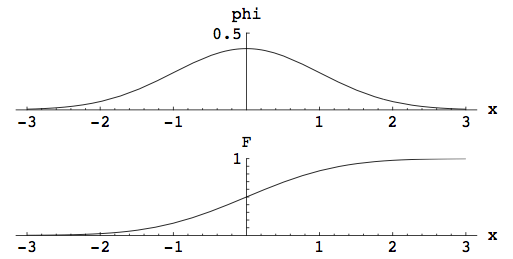
\includegraphics[width=8cm]{./bilder/normalverteilung.png}
		Dichtefunktion (oben) und Verteilungsfunktion (unten) der Normalverteilung. 
   		\end{minipage} \\ 
	$ 68\% $ der Werte liegen im Intervall $[ \mu - \sigma, \mu + \sigma]$, 
	$95\% $ in $[ \mu - 2\sigma, \mu + 2\sigma]$, 	
	$99.7\% $ in $[ \mu - 3\sigma, \mu + 3\sigma]$
		\vspace{5mm}
	


\newpage

	\subsection{Zentraler Grenzwertsatz \skript{107} \sachs{127}}
      	$X_1, X_2, \ldots , X_n$ sind lauter identisch verteilte (nicht notwendig normalverteilt!)
      	unabhängige Zufallsvariablen mit demselben Erwartungswert $\mu$ und derselben Varianz $\sigma^2$.
      	\\ 
      	Dann hat die Summe ($S_n = \sum_{i=1}^n X_i$) den Erwartungswert $n \mu$ und die Varianz
      	$n \sigma^2$. \\
      	Die damit verbundene standardisierte ($E(X) = 0, var(X) = 1$) Variable $Z_n$ ist somit wie
      	folgt definiert: \\ $ Z_n = \dfrac{S_n - n \mu}{\sqrt{n} \sigma} = \dfrac{\overline{X} - \mu}{\sigma
      	/ \sqrt{n}}$
      	\\
      	Für $\boldsymbol{n \to \infty}$ strebt die Verteilung von $Z_n$ gegen die
      	Standardnormalverteilung. \\
        
\hrule

	\subsection{Exponentialverteilung \skript{96}}
 		\begin{minipage}{10cm}
		Zur Ermittlung der Dauer von zufälligen Zeitintervallen ohne Gedächnis
		(W'keit, dass X in der nächsten Minute defekt geht = const.). Beispiele :
		\begin{itemize}
          \item Lebensdauer von Atomen beim radioaktiven Zerfall
          \item Lebensdauer von Bauteilen, Maschinen \& Geräten\\(MTBF -
          Mean Time Before Failure = $\frac{1}{\lambda}$)
        \end{itemize}
        
		\underline{Dichtefunktion und Verteilungsfunktion}\\
        $\varphi(x)=\begin{cases}
		\lambda e^{-\lambda x}  & x \geq 0\\
  		0						& x < 0
		\end{cases}$
		
		$F(x)=\begin{cases}
  		1-e^{-\lambda x}  		& x \geq 0\\
  		0	 					& x < 0
		\end{cases}$\\ \\

		\underline{Erwartungswert und Varianz}\\
		$E(X)=\frac{1}{\lambda}$\\
		$var(X)=\frac{1}{\lambda^2}$ \\
        \end{minipage}
		\begin{minipage}{8cm}
        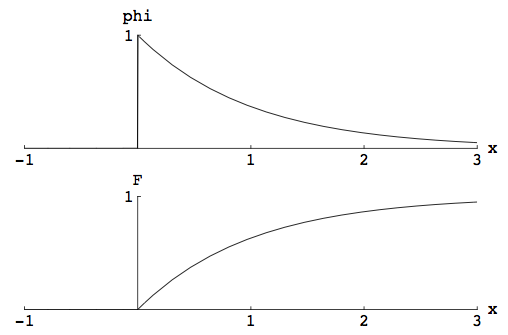
\includegraphics[width=8cm]{./bilder/exponentialverteilung.png}
		Dichtefunktion (oben) und Verteilungsfunktion (unten) der Exponentialverteilung.
        \end{minipage}
		

\hrule

	\subsection{Hypergeometrische Verteilung \skript{120} \sachs{117}}
		\begin{minipage}{13cm}
        Ist die Wahrscheinlichkeit dass in einer $m$ Elemente umfassenden 
		Stichprobe aus einer Grundgesamtheit von $n$ Elementen, von denen $r$ eine
		spezielle Eigenschaft besitzen, $k$ Elemente mit der Eigenschaft zu
		finden sind.\\
		\vspace{5mm} 
		$p(k)=P(X=k)=\dfrac{\binom r k \binom{n-r}{m-k}}{\binom n m}$ 
        \hspace{10mm} für $0\leq k \leq r$ und $k \leq n$\\
        Erwartungswert: \hspace{10mm} $E(X)=m \dfrac{r}{n}$\\
        Varianz: \hspace{22mm} $var(X)=m \dfrac{r(n-r)(n-m)}{n^2(n-1)}$
        \end{minipage}
		\begin{minipage}{5cm}
        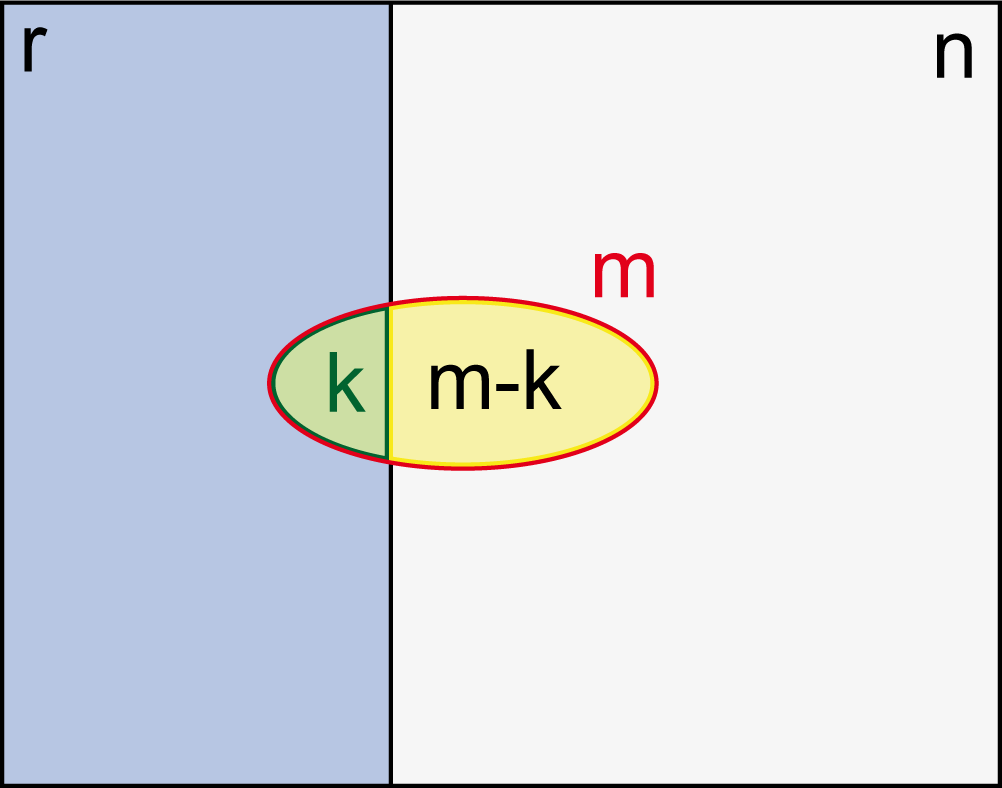
\includegraphics[width=5cm]{./bilder/hypergeo.png}
        \end{minipage}
		
		\vspace{3mm}
		{\bf Beispiel:} Lotto, $n=45$ Zahlen, $r=6$ (die gezogenen Zahlen), $m=6$
		(meine Zahlen)\\
		$P(X=4)=P(Ein Vierer)=\dfrac{\binom 6 4 \binom {39} 2}{\binom {45}
		6}=0.001364$
\newpage

		\subsection{Poissonverteilung \skript{121} \sachs{115}}
		\begin{tabular}{ll}
        $P_\lambda(k)=\frac{\lambda^k}{k!}e^{-\lambda}$\\
        Erwartungswert: \hspace{10mm} $E(X)=\lambda$\\
        Varianz: \hspace{22mm} $var(X)=\lambda$
        \vspace{2mm}\\
        {\bf Anwendung der Poisson-Verteilung:} für die Häufigkeiten seltener
        Ereignisse. Anzahl Anrufe bei einer Telefonzentrale \\ in einer gewissen
        Periode. Anzahl grosse Versicherungsschäden in einer gewissen Periode.
        Anzahl Jobs, die bei einem Server \\ ankommen. Anzahl Ereignisse in
        einem Zeitintervall. Anzahl Lokomotiven der SBB, die in der nächsten Woche 
        einen Defekt \\ haben. Anzahl der Gewinner mit 4 Richtigen im Lotto.
        \end{tabular}

\hrule

		\subsection{Binomialverteilung \skript{117} \sachs{112}}
		\begin{tabular}{p{18cm}}
    	Wird angewendet bei einem Experiment mit nur zwei Ausgängen (Ereignis mit W'keit $p$ tritt
    	ein, Ereignis tritt nicht ein). \\
    	Eine Zufallsvariable mit diskreten Werten $k \in \{
    	0,\ldots,n \}$ heisst binomialverteilt zum Parameter $p$, wenn die
        Wahrscheinlichkeit des Wertes $k$ wie folgt ist:
        %\end{tabular}
		%\begin{center}
		$$X = Bi(n; p) = \binom n k p^k(1-p)^{n-k} \qquad \mu = E(X) = p \cdot n \qquad \sigma^2 =
		var(X) = n \cdot p (1-p)$$
		%\end{center}
		%\begin{tabular}{ll} 
		
		$n$: Versuche \hspace{10mm}
		$k$: k-mal erfolgreich \hspace{10mm}
		$p$: Wahrscheinlichkeit\\\\
		
		{\bf Beispiel:} Wie hoch ist die Wahrscheinlichkeit, dass bei 350 Leuten genau
		k $(k\leq 350)$ heute Geburtstag haben?\\
		$P(k)=\binom {350} k \left(\frac{1}{365}\right)^k
		\left(\frac{364}{365}\right)^{350-k}$
		
        \end{tabular}


\hrule
		\subsection{Gleichverteilung}
		\begin{tabular}{p{9cm} p{9cm}}
        %$M_n=\frac{X_1+\ldots+X_n}{n}$ \hspace{10mm} $M_n$: Mittelwert\\
		\textbf{Stetig \skript{93}} 
		& \textbf{Diskret \skript{116}} \\
		Erwartungswert: $E(X)=\frac{a + b}{2}$
		& Erwartungswert: $E(X)=\frac{n + 1}{2}$\\
		Varianz: $var(X)=\frac{(b-a)^2}{12}$
		& Varianz: $var(X)=\frac{n^2-1}{12}$
        \end{tabular}
\vspace{1mm}
\hrule

\section{Schätzen skript{127} \sachs{134}}

	\subsection{Konsistente Schätzer \skript{129} \sachs{136}}
		Ein Schätzer ist konsistent, wenn $\lim \limits_{n \rightarrow \infty}$ = E(X)
		ergibt\\
		\begin{tabular}{p{10cm}p{8cm}}
        Der Mittelwert der Stichprobe ist ein konsistenter Schätzer.
        & $\lim\limits_{n\to\infty}=\frac{X_1+\ldots+X_n}{n}=E(X)$
        \end{tabular}

        \hspace*{2.1mm}Der Schätzer $\bar{X}=\frac{X_1+\ldots +X_n}{n}$ heisst
        der Stichprobenmittelwert der Stichprobe $X_1,\ldots,X_n$. \\        
       
         {\bf Mit Taschenrechner:} $ \qquad \bar{X}$: \texttt{mean(\{$X_1,\ldots,X_i$\}) \\}
        
\hrule

	\subsection{Erwartungstreue Schätzer \skript{129} \sachs{136}}
		Ein Schätzer ist erwartungstreu, wenn $E($Schätzer$)=E($realer Wert$)$\\
		\begin{tabular}{p{8cm}p{10cm}}
        Ist der Stichprobenmittelwert ein konsistenter Schätzer, aber er ist
        sogar erwartungstreu:
        & $E(\mu(X_1,\ldots,X_n))=\frac{E(X_1)+\ldots+E(X_n)}{n}=E(X)$\\
        Erwartungstreue Schätzer für $var(x)$ ist:\\
        $S^2=\frac{1}{n-1}(\sum X_i^2-\frac{1}{n}(\sum X_i)^2)$
        & Stichprobenvarianz, empirische Varianz\\
        $S^2=\frac{1}{n-1}\sum\limits_{i=1}^n(X_i-\bar{X})^2$
        & $\bar{X}=M_n$ heisst Stichprobenmittelwert\\ \\
        {\bf Mit Taschenrechner}\\
        \multicolumn{2}{l}{$S^2$: \texttt{variance(\{$X_1,\ldots,X_i$\})} \qquad $S$: \texttt{stdDev(\{$X_1,\ldots,X_i$\}) }}
        \end{tabular}
	\subsubsection{Kleinstmöglicher Fehler}
		$E( (E(X)- \frac{x_1+\ldots+x_n}{n})^2)= minimal$

\newpage
	\subsection{Maximum Likelihood Schätzer \skript{131}}
	Sinn des Likelihoodschäzers ist einen unbekannten Parameter $\vartheta$ einer Dichtefunktion
	$\phi(x, \vartheta)$ zu schätzen.
	
	$$L(x_1,\ldots,x_n;\vartheta)=\phi(x_1,\vartheta)\ldots \phi(x_n,\vartheta) \quad \Longrightarrow \quad
	\frac{d}{d \vartheta} L(x_1,\ldots,x_n;\vartheta) = 0 \quad \Longrightarrow \quad \vartheta = ? 
	\text{	(Maximum-Likelihood-Schätzer})$$
	
	Für eine normalverteilte Grösse lautet die Likelihood Funktion:
	$L(x_1,\ldots,x_n;\vartheta)=\frac{1}{(\sqrt2\pi)^n}e^{-\frac{1}{2\sigma^2}\sum\limits_{i=1}^n (x_i-\vartheta)^2}$\ 

	Der unbekannte Parameter $\vartheta$ kann nun durch suchen des Maximums der Funktion ermittelt
	werden ($\vartheta$ wird variert). Die Funktion wird maximal, wenn die Summe im
	Exponent minimal wird. Das $\vartheta$, das die Summe minimiert, kann durch
	\textbf{ableiten nach $\vartheta$ und null setzen ermittelt} werden. Es können
	auch Stichprobenvarianz $S^2$ oder Ähnliches ermittelt werden. \\
	
\hrule

	\subsection{t-Verteilung \sachs{150}}
	Der Mittelwert ($\frac{x_1+\ldots+x_n}{n}$) normalverteilter Daten ist
    t-Verteilt, wenn die \textbf{Varianz mit der Stichprobenvarianz geschätzt} wurde.\\
    Ab einer gewissen Anzahl Messungen ($n \geq 30$) kann näherungsweise auch wieder mit
    der Normalverteilung gerechnet werden.  \\ \\
	\begin{tabular}{p{10cm}p{8cm}}
    Die Wahrscheinlichkeitdichte der
    t-Verteilung ist: &$\varphi_t(t)=\frac{\Gamma (\frac{k+1}{2})}{\sqrt{\pi
    k}\Gamma(\frac{k}{2})}\left(1+\frac{t^2}{k}\right)^{- \frac{k+1}{2}}$\\ \\
    Falls Verteilung bekannt ist, finde t so dass
    &$P\left(\left|\frac{\bar{X}-\mu}{S / \sqrt{n}}\right|\leq t\right) = 1 - \alpha$\\ \\
    &$\mu\in\left[\bar{X}-t\frac{S}{\sqrt{n}},\bar{X}+t\frac{S}{\sqrt{n}}\right]$\\
    \end{tabular}\\
	\begin{minipage}{10cm}
 		\subsubsection{Checkliste}
		\begin{tabular}{ll}
        1) $\bar{X}, S$ als Schätzungen von $\mu, \sigma$ ermitteln\\
        2) $t$ aus {\em t-Tabelle} $(k=n-1)$ für $\alpha$ = Fehlerw'keit\\
        3) Intervall
        $\left[\bar{X}-t\frac{S}{\sqrt{n}},\bar{X}+t\frac{S}{\sqrt{n}}\right]$,
        $(1-\alpha)$ Konfidenzintervall
        \end{tabular}\\
		\subsubsection{Anwendung}
		\begin{tabular}{ll}
        $\frac{\textcolor{red}{\bar{X}}-\mu}{\textcolor{blue}{S}/\sqrt{\textcolor{green}{n}}}$
        & t-Verteilt\\ \\
        \end{tabular}
    
    \end{minipage}
	\begin{minipage}{10cm}
   		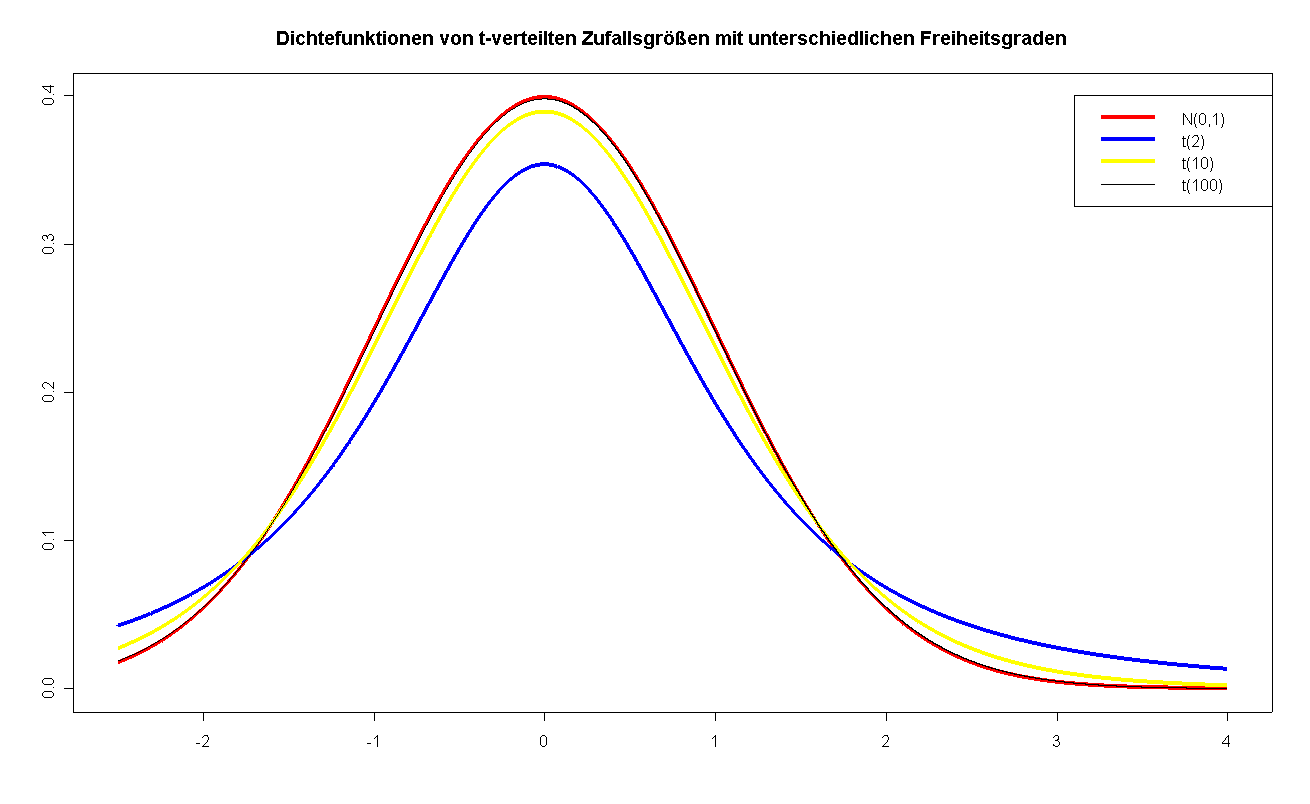
\includegraphics[width=8cm,height=4cm]{./bilder/T-Verteilung.png}\\
		$\lim \limits_{x\rightarrow \infty}$ = 0 aber langsamer wie bei
		Gaussverteilung 
    \end{minipage}

		\begin{tabular}{p{2cm}p{16cm}}
        Beispiel: & \textcolor{green}{10} Messungen ergeben Durchschnittswert
        \textcolor{red}{4{,}7} und eine Standardabweichung \textcolor{blue}{0{,}1}.
        Finde ein 99\%  Konfidenzintervall für $\mu$.\\
        
         Finde t: & \begin{tabular}{| c | c | c | c |}
                   \hline
                   $k=\textcolor{green}{n}-1$ & \ldots & 0{,}995\\
                   \hline
                   \vdots & \vdots & \vdots \\
                   \hline
                   9 & \ldots & 3{,}2498\\
                   \hline
                   \end{tabular}
        
       		 $\left[\textcolor{red}{\bar{X}}-3,2498\frac{\textcolor{blue}{S}}{\sqrt{\textcolor{green}{n}}},
		\textcolor{red}{\bar{X}}+3,2498\frac{\textcolor{blue}{S}}{\sqrt{\textcolor{green}{n}}}\right]
		\Rightarrow 
		\left[{\color{red}4{,}7}-3{,}2498\frac{\textcolor{blue}{0{,}1}}{\sqrt{\textcolor{green}{10}}},
		\textcolor{red}{4{,}7}+3{,}2498\frac{\textcolor{blue}{0{,}1}}{\sqrt{\textcolor{green}{10}}}\right]$\\ \\
		& $\mu\in \left[4{,}5072, 4{,}8028\right]$ mit Wahrscheinlichkeit 99\%
        \end{tabular}
\hrule

	\subsection{Konfidenzintervall \skript{139} \sachs{146}}
	\begin{tabular}{p{18cm}}
     Ein Intervall $[L(X_1,\ldots,X_n),R(X_1,\ldots,X_n)]$ heisst ein
     $1-\alpha$- Konfidenzintervall für den Parameter $\vartheta$, wenn der wahre
     Wert des Parameters $\vartheta$ höchstens mit Wahrscheinlichkeit $\alpha$
     ausserhalb des Intervalls liegt.
    \end{tabular}\\

\newpage
\section{Hypothesentest skript{143} \sachs{162}}
	\subsection{Grundsätze}
	- ``Man braucht Aussagen, die man widerlegen könnte.''\\
	- Irrtum ist möglich (Irrtumsw'keit $\alpha$)\\
	- Beweis durch Widerlegen des Gegenbeweises
	\subsection{Vorgehen}
	\begin{enumerate}
      \item Hypothese, die der Test Widerlegen soll
      \item Irrtumsw'keit $\alpha$ = 0.05, 0.01, \ldots (Niveau=1-$\alpha$)
      \item Testgrösse T, W'keitsverteilung
      \item Bestimmung der Schranken t für: $P(|T-E(T)|>t)=\alpha$
      \item Falls Messungen ergeben $|T-E(T)|>t \Longrightarrow$ Hypothese
      falsch mit W'keit 1- $\alpha$
    \end{enumerate}
    
    
	\subsection{$\chi^2$-Test - Testen einer Wahrscheinlichkeitsverteilung
	\skript{147} \sachs{174}}
		$\chi ^2 = Z_1^2+\ldots+Z_r^2$ ($Z_r$ sind standardnormalverteilt) $\Longrightarrow
		\chi^2$-Verteilung mit r-Freiheitsgraden\\ \\
		\begin{minipage}{6.5cm}
        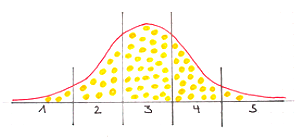
\includegraphics[width=6cm]{./bilder/chi_quadrat.png}\\
        \end{minipage}
		\begin{minipage}{12cm}
        Teilintervalle: $I_i$, $i=1,\ldots,k$\\
        Wahrscheinlichkeit: $P(X\in I_i)=\textcolor{red}{p_i}$\\
        $n$ Beobachtungen, davon jeweils \textcolor{blue}{$n_i$} im Intervall
        $i$ ($n=\sum n_i$)\\
        $D=\sum\limits_i\frac{(\textcolor{blue}{n_i}-\textcolor{red}{np_i})^2}{\textcolor{red}{np_i}}$
        \hspace{8mm} ist $\chi^2_{k-1}$, mit $k-1$ Freiheitsgrade\\
        $\varphi_n(x)=  \begin{cases}\displaystyle \frac{x^{\frac{r}{2}-1}e^{
        -\frac{x}{2}}}{2^{\frac{r}{2}}\Gamma\left(\frac{r}{2}\right)} & x>0 \\
        0 & x\leq 0 \end{cases} $\\  
		$E(X)=r; \quad var(X)=2r$
        \end{minipage}
		
		\subsubsection{Durchführung des $\chi^2$-Tests}
		\begin{minipage}{13cm}
		\begin{tabular}{p{4cm}p{8cm}}
        1. Klasse bilden: & Gross genug, dass mehrere Beobachtungen in jede
        Klasse fallen.\\  
        & (erste und letzte Klasse können breiter sein)\\
        & Faustregel: $\boldsymbol{n_i\geq 5}$; k: Anzahle der Klassen\\
        2. \textbf{Diskrepanz $D$} berechnen & \begin{tabular}[t]{|c|c|c|c|c|}
                                  \hline
                                  $i$ & Intervall & $p_i$ & $n_i$ &
                                  $(n_i-np_i)^2/np_i$\\
                                  \hline
                                  1 & & & & \\
                                  2 & & & & \\
                                  3 & & & & \\
                                  4 & & & & \\
                                  5 & & & & \\
                                  \hline
                                  & & & & $D=\sum$ \\
                                  \hline
                                  
                                  \end{tabular}\\
        3. Schwellenwert für $D$ & aus $\chi_{k-1}^2$-Tabelle lesen. Wenn
        $\alpha$ nicht vorgegeben, dann $\alpha$ z.B. $0.1$ oder $0.05$
        wählen.\\
        &(Anzahl Freiheitsgrade)= Anzahl Klassen $ -1 $ = $k - 1$ \\ & $p=1-\alpha$ \hspace{10mm}$\alpha=$Irrtumswahrscheinlichkeit\\
        & \textcolor{green}{$D \geq D_{1-\alpha}$} Hypothese ist unwahrscheinlich!\\
        & $D < D_{1-\alpha}$ Hypothese nicht wiederlegbar!\\
        & \textcolor{blue}{$D \leq D_\alpha$} Daten möglicherweise
        ''fabriziert''!\\
        \end{tabular}
        \end{minipage}
		\begin{minipage}{6cm}
        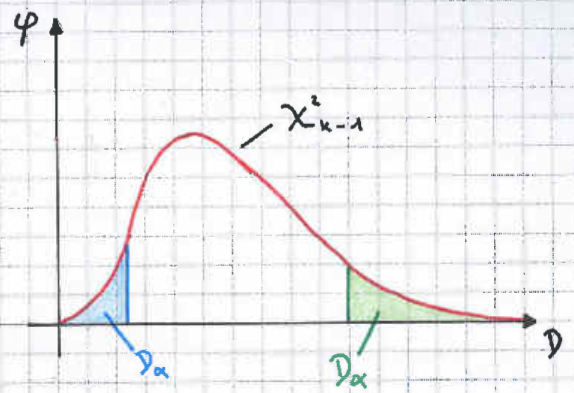
\includegraphics[width=6cm]{./bilder/chi-test.png}
        \end{minipage}\\
	\begin{tabular}{ll}
    	Nachteile:&	-Grob verpixeltes Bild der Verteilung\\
    	&			-wenn wenig Messwerte $\Longrightarrow$ geringe Aussagekraft
    \end{tabular}

\newpage
	\subsection{Kolmogorov-Smirnov Test \skript{149}}
	\begin{tabular}{ll}
    Idee: & Vergleiche Verteilungsfunktionen (statt der Dichtefunktionen)\\
    Daten: & $X$ Zufallsvariable, Verteilungsfunktion $F_x$, $n$ Messungen
    ergeben Stichprobe $x_i$
    \end{tabular}

	\begin{minipage}{6cm}
    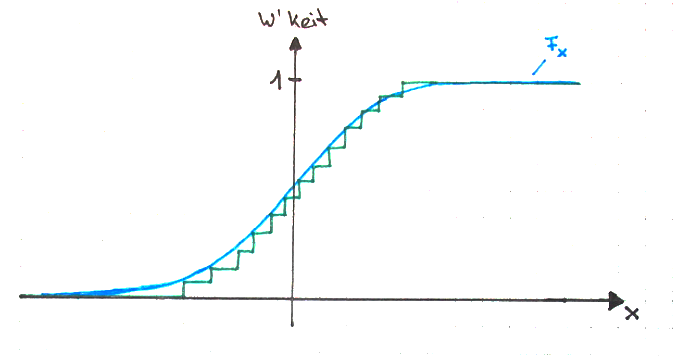
\includegraphics[width=6cm]{./bilder/ks1.png}\\
    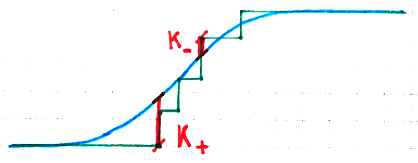
\includegraphics[width=6cm]{./bilder/ks2.png}\\
    \end{minipage}
	\begin{minipage}{12cm}
    \textcolor{blue}{$F_x$ theoretische Verteilungsfunktion}\\ \\
    \vspace{15mm}
    \textcolor{green}{empirische Verteilungsfunktion $\frac{Anzahl\{x_i \leq
    x \}}{n}$}\\

    \textcolor{red}{$K_-$ = max}
    \textcolor{blue}{$(F_x$(x)} -
    \textcolor{green}{$F_{emp}$(x))} 
    $\cdot\sqrt{n}$ \\
    \textcolor{red}{$K_{+}$ = max} 
    \textcolor{green}{$(F_{emp}(x)$}-
    \textcolor{blue}{$F_x(x))$}
    $\cdot\sqrt{n}$ \\

    \end{minipage}

	\begin{tabular}{p{18cm}}
		Sei $X1,\ldots,Xn$ sei eine Stichprobe einer Zufallsvariable $X$ . Der
		Kolmogorov- Smirnov-Test auf dem Niveau $\alpha$ für die Hypothese, 
		dass $X$ die Verteilungsfunktion $F$ hat wird wie folgt durchgeführt: \\ \\
		1. Berechne 
		$K_n^+ = \sqrt{n} \underset{-\infty<x<\infty}{max}(F(x)-F_n(x))$ und
		$K_n^- = \sqrt{n} \cdot \underset{x \in \mathbb{R}}{max}(F_n(x)-F(x))$  \\
		2. Finde $t_{n,1-\alpha}$ in der Tabelle\\ 
		3. Falls $K^+_n > t_{n,1-\alpha}$ oder $K^-_n < t_{n,\alpha}$,
		verwerfe die Hypothese, dass $X$ die Verteilungsfunktion $F$ hat. 
	\end{tabular}

\section{Wichtige Formeln}
\subsection{Reihenentwicklungen}
\renewcommand{\arraystretch}{2.5}
\begin{tabular}{llll}
\textbf{Geometrische Reihe}
	& $\sum\limits_{n=0}^{\infty} x^n$ 
	& $= \dfrac{1}{1-x}$
	& $|x| < 1$ \\
	
	& $\sum\limits_{k=0}^{\infty} k \, x^k$ & $= x \sum\limits_{k=1}^{\infty} k \,
	x^{k-1} = \dfrac{x}{(1-x)^2} $ 
	& $x \neq 1$ \\
\textbf{Binominalreihe} 
	& $\sum\limits_{n=0}^\infty \binom{\alpha}{n} x^n $ &$= (1+x)^\alpha$
	& $x \in (-1,1)$ \\
\textbf{E-Funktion}
	& $\sum\limits_{k = 0}^{\infty} \dfrac{x^k}{k!}$ &$ = e^x$
	& 
\end{tabular}
\renewcommand{\arraystretch}{1}

\newpage

\section{Übungsverzeichnis}
\begin{center}
\begin{tabular}{|l|l|l|}
\hline
\textbf{Titel} & \textbf{Beschreibung} & \textbf{Übungsnummer} \\ \hline
$\chi^2$-Test & M\&M's Experiment & 12.1 \\ \hline
4 Damen und 5 Her. auf 9 Stühle Platz. & Verschiedene Ereignisse die Auftreten auflisten & 3.1 \\ \hline
Alzheimer-Test & Bedingte W'keit, Satz der totalen W'keit & 2.4 \\ \hline
Auto-Ziegen-Problem & Monty-Hall Problem & 4.1, 4.2, 4.3 \\ & & 5.1 (mit Gewinn) \\ \hline
Beweis Poisson-Verteilung & Bewieiss, dass PV wirklich eine W'keitsverteilung ist & 10.2 \\ \hline
Buch mit n Seiten und f Druckfehlern & Poisson-Verteilung, W'keit genau 2 Fehler auf einer Seite & 10.1 \\ \hline
Dichtefunktion mit unb. Parameter & Parameter, $F(x)$, $E(x)$, $Var(x)$ und Abw. von $E(x)$ berech. & 7.3, 10.4 \\ \hline
Epidemie auf Kleinplanet Zürch & ein paar der infiz. Bewohner werden untersucht & 3.5 \\ \hline
EW einer sym. Dichtefunktion & & 7.2 \\ \hline
Exp.verteilte ZV mit unb. Parameter & $Var(x)$ berechnen & 8.1 \\ \hline
Faire Münze mehrmals werfen & W'keiten der möglichen Werte und $E(x)$ berechnen & 5.3 \\ \hline 
Faire Münze mit Gewinn & Gewinn entspricht der (k+1)-ten Primzahl & 5.2 \\ \hline
Fairer Würfel n mal geworfen & W'keit mehr als 15 von 100 6er abzuweichen & 10.5 \\ \hline
Familie mit Kindern & Versch. Ereignisse die Auftreten auflisten & 2.2 \\ \hline
Funktionsf. eines Gerätes (krit. Bauteil) & Ausfall des Bauteils inn. der ersten Woche & 8.3 \\ \hline
Game-Controller & Schätzwert für Drehgeschwindigkeit & 13.2 \\ \hline
Gleichverteilte Zufallsvariable & Erwartungswert und Verteilungsfunktion berechnen & 7.4 \\ \hline
Gleichverteilte ZV & Intervall [0,1], $F(x)$, $\varphi(x)$, $E(x) $ und $var(x)$ & 8.2 \\ \hline
Glücksrad & Spielfolgen & 2.1 \\ \hline
Google-Matrix & Besuchsw'keiten anhand von Link-Struktur bestimmen & 4.5 \\ \hline
Hüte und Lose & 2 Hüte mit untersch. Lose und Nieten & 3.4 \\ \hline
Hypergeometrische Verteilung & Prozess wegen Diskriminierung & 12.3 \\ \hline
Hypotese Testen & Zahlen sollen angeblich Exponentialv. sein mit Parameter & 13.1 \\ \hline
Impfexperiment & W'keit, dass Individuum Komplik. hat, Poisson-Verteilung & 10.3 \\ \hline
Kalman-Filter & Konstruktion & 13.3, 13.4 \\ \hline
Kursteilnehmer in 4er-Gruppen eint. & vieviele versch. Arten gibt es & 3.3 \\ \hline
Laborversuch, geg. $Var(x)$ & Resultat soll bis zu einer Stelle nach dem Komma genau sein & 7.1 \\ \hline
M\&M's Experiment & $\chi^2$  Wird eine Fabe bevorzugt?  & 12.1 \\ \hline
Maschinene die Bauteile produziert & Maschinen produzieren untschersch. Ausschuss & 4.4 \\ \hline
Mengen & Visualisieren von Ereignissen & 1.1, 1.2 \\ \hline
Monty-Hall Problem & Auto-Ziegen-Problem & 4.1, 4.2, 4.3 \\ & & 5.1 (mit Gewinn) \\ \hline
Multiple Choice Test & 10 Fragen a je 3 Antworten & 3.5 \\ \hline
Numbers mit Morde in Grossstadt & & 11.1 \\ \hline
Prozess wegen Diskriminierung & hypergeometrische Verteilung & 12.3 \\ \hline
Raketenexperiment Müller & Meth. der kleins. Quad. um approx. der Datenp. zu kriegen & 9.6 \\ \hline
Schätzer finden & & 11.2 - 11.4 \\ \hline
Schätzer mit Param. der Exp.vert. & Schätzer entw. konsistend und/oder erwartungstreu & 11.2 \\ \hline
Sensor-, Server-Problem & Lineare Regression durchführen neue Werte zu finden & 6.6 \\ \hline
Sitzordnungen & vieviele Sitzordnungen bei n-Personen möglich sind & 3.2 \\ \hline
Sorte Körnermais liefert Ertrag & empirische Standardabweichung, 95\%-Quantile der Normalv. & 9.2 \\ \hline
Standardnormalvert. ZV& $P(-0.46 \leq X \leq 0.21)$ berechnen & 9.1 \\ \hline
Streng mon. Wachsende $F(x)$ & $F(x)$ einer anderen Zufallsvariablen berechenen & 7.5 \\ \hline
Unfaire Münze & n Würfe und daraus Erwartungswert und Varianz berechnen & 6.3 \\ \hline
Unfairer Würfel & Erwartungswert und Varianz der Augenzahl berechnene & 6.1 \\ \hline
Wahrscheinlichkeitsmaschine & generiert ganze Zufallszahlen >= 0 & 5.4 \\ \hline
Webseite mit Besucherzahlen & Hypothese und Normalverteilung & 12.2 \\ \hline
Wendep. der Normalv. bestimmem & $P(x_{-} \leq X \leq x_{+})$  berechnen & 9.5
\\ \hline Würfel wird n-mal geworfen & W'keit, dass bei $n=100$ die Augens. zwischen $320-360$ & 9.4 \\ \hline
Zementsäcke à $1$kg mit Standardabw. & W'keit dass Sack weniger wie 99.4 kg Inhalt hat & 9.3 \\ \hline
Zufallsvariable mit Werten 0 oder 1 & Erwartungswert und Varianz berechnen & 6.2 \\ \hline
\end{tabular}
\end{center}

\newpage

\section{Tabellen}
\copyright$\;$ Prof. Dr. Andreas Müller
\subsection{Quantilen der Normalverteilung}
	\begin{minipage}{18cm}
    	\centering
    	\scriptsize
\begin{tabular}{|l|r|}
\hline
$p$&$x$\\
\hline
0.75&0.6745\\
0.8&0.8416\\
0.9&1.2816\\
0.95&1.6449\\
0.975&1.9600\\
0.99&2.3263\\
0.995&2.5758\\
0.999&3.0902\\
0.9995&3.2905\\
\hline
\end{tabular}
    \end{minipage}

	\subsection{Verteilungsfunktion der Normalverteilung}
	\begin{minipage}{18cm}
    	\centering
        \scriptsize
\begin{tabular}{|r|rrrrrrrrrr|}
\hline
$x$&+0.00&+0.01&+0.02&+0.03&+0.04&+0.05&+0.06&+0.07&+0.08&+0.09\\
\hline
0.0&0.5000&0.5040&0.5080&0.5120&0.5160&0.5199&0.5239&0.5279&0.5319&0.5359\\
0.1&0.5398&0.5438&0.5478&0.5517&0.5557&0.5596&0.5636&0.5675&0.5714&0.5753\\
0.2&0.5793&0.5832&0.5871&0.5910&0.5948&0.5987&0.6026&0.6064&0.6103&0.6141\\
0.3&0.6179&0.6217&0.6255&0.6293&0.6331&0.6368&0.6406&0.6443&0.6480&0.6517\\
0.4&0.6554&0.6591&0.6628&0.6664&0.6700&0.6736&0.6772&0.6808&0.6844&0.6879\\
0.5&0.6915&0.6950&0.6985&0.7019&0.7054&0.7088&0.7123&0.7157&0.7190&0.7224\\
0.6&0.7257&0.7291&0.7324&0.7357&0.7389&0.7422&0.7454&0.7486&0.7517&0.7549\\
0.7&0.7580&0.7611&0.7642&0.7673&0.7704&0.7734&0.7764&0.7794&0.7823&0.7852\\
0.8&0.7881&0.7910&0.7939&0.7967&0.7995&0.8023&0.8051&0.8078&0.8106&0.8133\\
0.9&0.8159&0.8186&0.8212&0.8238&0.8264&0.8289&0.8315&0.8340&0.8365&0.8389\\
1.0&0.8413&0.8438&0.8461&0.8485&0.8508&0.8531&0.8554&0.8577&0.8599&0.8621\\
1.1&0.8643&0.8665&0.8686&0.8708&0.8729&0.8749&0.8770&0.8790&0.8810&0.8830\\
1.2&0.8849&0.8869&0.8888&0.8907&0.8925&0.8944&0.8962&0.8980&0.8997&0.9015\\
1.3&0.9032&0.9049&0.9066&0.9082&0.9099&0.9115&0.9131&0.9147&0.9162&0.9177\\
1.4&0.9192&0.9207&0.9222&0.9236&0.9251&0.9265&0.9279&0.9292&0.9306&0.9319\\
1.5&0.9332&0.9345&0.9357&0.9370&0.9382&0.9394&0.9406&0.9418&0.9429&0.9441\\
1.6&0.9452&0.9463&0.9474&0.9484&0.9495&0.9505&0.9515&0.9525&0.9535&0.9545\\
1.7&0.9554&0.9564&0.9573&0.9582&0.9591&0.9599&0.9608&0.9616&0.9625&0.9633\\
1.8&0.9641&0.9649&0.9656&0.9664&0.9671&0.9678&0.9686&0.9693&0.9699&0.9706\\
1.9&0.9713&0.9719&0.9726&0.9732&0.9738&0.9744&0.9750&0.9756&0.9761&0.9767\\
2.0&0.9772&0.9778&0.9783&0.9788&0.9793&0.9798&0.9803&0.9808&0.9812&0.9817\\
2.1&0.9821&0.9826&0.9830&0.9834&0.9838&0.9842&0.9846&0.9850&0.9854&0.9857\\
2.2&0.9861&0.9864&0.9868&0.9871&0.9875&0.9878&0.9881&0.9884&0.9887&0.9890\\
2.3&0.9893&0.9896&0.9898&0.9901&0.9904&0.9906&0.9909&0.9911&0.9913&0.9916\\
2.4&0.9918&0.9920&0.9922&0.9925&0.9927&0.9929&0.9931&0.9932&0.9934&0.9936\\
2.5&0.9938&0.9940&0.9941&0.9943&0.9945&0.9946&0.9948&0.9949&0.9951&0.9952\\
2.6&0.9953&0.9955&0.9956&0.9957&0.9959&0.9960&0.9961&0.9962&0.9963&0.9964\\
2.7&0.9965&0.9966&0.9967&0.9968&0.9969&0.9970&0.9971&0.9972&0.9973&0.9974\\
2.8&0.9974&0.9975&0.9976&0.9977&0.9977&0.9978&0.9979&0.9979&0.9980&0.9981\\
2.9&0.9981&0.9982&0.9982&0.9983&0.9984&0.9984&0.9985&0.9985&0.9986&0.9986\\
3.0&0.9987&0.9987&0.9987&0.9988&0.9988&0.9989&0.9989&0.9989&0.9990&0.9990\\
\hline
\end{tabular}
    \end{minipage}

	\subsection{Quantilen für den Kolmogorov-Smirnov-Test}
	\begin{minipage}{18cm}
    	\centering
    	\scriptsize
\begin{tabular}{|r|rrr|rrr|rrr|}
\hline
$n$&$p=0.01$&$p=0.05$&$p=0.1$&$p=0.25$&$p=0.5$&$p=0.75$&$p=0.9$&$p=0.95$&$p=0.99$\\
\hline
1&0.01000&0.05000&0.10000&0.25000&0.50000&0.75000&0.90000&0.95000&0.99000\\
2&0.01400&0.06749&0.12955&0.29289&0.51764&0.70711&0.96700&1.09799&1.27279\\
3&0.01699&0.07919&0.14714&0.31117&0.51469&0.75394&0.97828&1.10166&1.35889\\
4&0.01943&0.08789&0.15899&0.32023&0.51104&0.76419&0.98531&1.13043&1.37774\\
5&0.02152&0.09471&0.16750&0.32490&0.52449&0.76741&0.99948&1.13916&1.40242\\
6&0.02336&0.10022&0.17385&0.32717&0.53193&0.77028&1.00520&1.14634&1.41435\\
7&0.02501&0.10479&0.17873&0.32804&0.53635&0.77552&1.00929&1.15373&1.42457\\
8&0.02650&0.10863&0.18256&0.32802&0.53916&0.77971&1.01346&1.15859&1.43272\\
9&0.02786&0.11191&0.18560&0.32745&0.54109&0.78246&1.01731&1.16239&1.43878\\
10&0.02912&0.11473&0.18803&0.32975&0.54258&0.78454&1.02016&1.16582&1.44397\\
11&0.03028&0.11718&0.19000&0.33304&0.54390&0.78633&1.02249&1.16885&1.44837\\
12&0.03137&0.11933&0.19160&0.33570&0.54527&0.78802&1.02458&1.17139&1.45207\\
13&0.03239&0.12123&0.19291&0.33789&0.54682&0.78966&1.02649&1.17357&1.45527\\
14&0.03334&0.12290&0.19396&0.33970&0.54856&0.79122&1.02823&1.17552&1.45810\\
15&0.03424&0.12439&0.19482&0.34122&0.55002&0.79259&1.02977&1.17728&1.46060\\
16&0.03509&0.12573&0.19552&0.34250&0.55123&0.79377&1.03113&1.17888&1.46283\\
17&0.03589&0.12692&0.19607&0.34360&0.55228&0.79482&1.03237&1.18032&1.46483\\
18&0.03665&0.12799&0.19650&0.34454&0.55319&0.79578&1.03351&1.18162&1.46664\\
19&0.03738&0.12895&0.19684&0.34535&0.55400&0.79667&1.03457&1.18282&1.46830\\
20&0.03807&0.12982&0.19709&0.34607&0.55475&0.79752&1.03555&1.18392&1.46981\\
30&0.04354&0.13510&0.20063&0.35087&0.56047&0.80362&1.04243&1.19164&1.48009\\
50&0.05005&0.13755&0.20794&0.35713&0.56644&0.80988&1.04933&1.19921&1.48969\\
100&0.05698&0.14472&0.21370&0.36331&0.57269&0.81634&1.05627&1.20666&1.49864\\
200&0.06049&0.14887&0.21816&0.36784&0.57725&0.82099&1.06117&1.21180&1.50458\\

\hline
\end{tabular}

    \end{minipage}
\newpage

	\subsection{Quantilen der t-Verteilung}
	\begin{minipage}{18cm}
    	\centering
    	\scriptsize
 \begin{tabular}{|r|rrrrrrr|}
\hline
$k = n-1$&0.75&0.8&0.9&0.95&0.975&0.99&0.995\\
\hline
1&1.0000&1.3764&3.0777&6.3138&12.7062&31.8205&63.6567\\
2&0.8165&1.0607&1.8856&2.9200&4.3027&6.9646&9.9248\\
3&0.7649&0.9785&1.6377&2.3534&3.1824&4.5407&5.8409\\
4&0.7407&0.9410&1.5332&2.1318&2.7764&3.7469&4.6041\\
5&0.7267&0.9195&1.4759&2.0150&2.5706&3.3649&4.0321\\
6&0.7176&0.9057&1.4398&1.9432&2.4469&3.1427&3.7074\\
7&0.7111&0.8960&1.4149&1.8946&2.3646&2.9980&3.4995\\
8&0.7064&0.8889&1.3968&1.8595&2.3060&2.8965&3.3554\\
9&0.7027&0.8834&1.3830&1.8331&2.2622&2.8214&3.2498\\
10&0.6998&0.8791&1.3722&1.8125&2.2281&2.7638&3.1693\\
11&0.6974&0.8755&1.3634&1.7959&2.2010&2.7181&3.1058\\
12&0.6955&0.8726&1.3562&1.7823&2.1788&2.6810&3.0545\\
13&0.6938&0.8702&1.3502&1.7709&2.1604&2.6503&3.0123\\
14&0.6924&0.8681&1.3450&1.7613&2.1448&2.6245&2.9768\\
15&0.6912&0.8662&1.3406&1.7531&2.1314&2.6025&2.9467\\
16&0.6901&0.8647&1.3368&1.7459&2.1199&2.5835&2.9208\\
17&0.6892&0.8633&1.3334&1.7396&2.1098&2.5669&2.8982\\
18&0.6884&0.8620&1.3304&1.7341&2.1009&2.5524&2.8784\\
19&0.6876&0.8610&1.3277&1.7291&2.0930&2.5395&2.8609\\
20&0.6870&0.8600&1.3253&1.7247&2.0860&2.5280&2.8453\\
21&0.6864&0.8591&1.3232&1.7207&2.0796&2.5176&2.8314\\
22&0.6858&0.8583&1.3212&1.7171&2.0739&2.5083&2.8188\\
23&0.6853&0.8575&1.3195&1.7139&2.0687&2.4999&2.8073\\
24&0.6848&0.8569&1.3178&1.7109&2.0639&2.4922&2.7969\\
25&0.6844&0.8562&1.3163&1.7081&2.0595&2.4851&2.7874\\
26&0.6840&0.8557&1.3150&1.7056&2.0555&2.4786&2.7787\\
27&0.6837&0.8551&1.3137&1.7033&2.0518&2.4727&2.7707\\
28&0.6834&0.8546&1.3125&1.7011&2.0484&2.4671&2.7633\\
29&0.6830&0.8542&1.3114&1.6991&2.0452&2.4620&2.7564\\
30&0.6828&0.8538&1.3104&1.6973&2.0423&2.4573&2.7500\\
50&0.6794&0.8489&1.2987&1.6759&2.0086&2.4033&2.6778\\
100&0.6770&0.8452&1.2901&1.6602&1.9840&2.3642&2.6259\\
500&0.6750&0.8423&1.2832&1.6479&1.9647&2.3338&2.5857\\
$10^3$&0.6747&0.8420&1.2824&1.6464&1.9623&2.3301&2.5808\\
$10^4$&0.6745&0.8417&1.2816&1.6450&1.9602&2.3267&2.5763\\
$10^5$&0.6745&0.8416&1.2816&1.6449&1.9600&2.3264&2.5759\\
$10^6$&0.6745&0.8416&1.2816&1.6449&1.9600&2.3264&2.5758\\
\hline
\end{tabular}
    \end{minipage}


	\subsection{Quantilen der $\chi^2$-Verteilung}
	\begin{minipage}{18cm}
    \scriptsize
\begin{center}
\begin{tabular}{|r|rrr|rrr|rrr|}
\hline
\strut$k = n-1$&$p=0.01$&$p=0.05$&$p=0.1$&$p=0.25$&$p=0.5$&$p=0.75$&$p=0.9$&$p=0.95$&$p=0.99$\\
\hline
1&0.000&0.004&0.016&0.102&0.455&1.323&2.706&3.841&6.635\\
2&0.020&0.103&0.211&0.575&1.386&2.773&4.605&5.991&9.210\\
3&0.115&0.352&0.584&1.213&2.366&4.108&6.251&7.815&11.345\\
4&0.297&0.711&1.064&1.923&3.357&5.385&7.779&9.488&13.277\\
5&0.554&1.145&1.610&2.675&4.351&6.626&9.236&11.070&15.086\\
6&0.872&1.635&2.204&3.455&5.348&7.841&10.645&12.592&16.812\\
7&1.239&2.167&2.833&4.255&6.346&9.037&12.017&14.067&18.475\\
8&1.646&2.733&3.490&5.071&7.344&10.219&13.362&15.507&20.090\\
9&2.088&3.325&4.168&5.899&8.343&11.389&14.684&16.919&21.666\\
10&2.558&3.940&4.865&6.737&9.342&12.549&15.987&18.307&23.209\\
11&3.053&4.575&5.578&7.584&10.341&13.701&17.275&19.675&24.725\\
12&3.571&5.226&6.304&8.438&11.340&14.845&18.549&21.026&26.217\\
13&4.107&5.892&7.042&9.299&12.340&15.984&19.812&22.362&27.688\\
14&4.660&6.571&7.790&10.165&13.339&17.117&21.064&23.685&29.141\\
15&5.229&7.261&8.547&11.037&14.339&18.245&22.307&24.996&30.578\\
16&5.812&7.962&9.312&11.912&15.338&19.369&23.542&26.296&32.000\\
17&6.408&8.672&10.085&12.792&16.338&20.489&24.769&27.587&33.409\\
18&7.015&9.390&10.865&13.675&17.338&21.605&25.989&28.869&34.805\\
19&7.633&10.117&11.651&14.562&18.338&22.718&27.204&30.144&36.191\\
20&8.260&10.851&12.443&15.452&19.337&23.828&28.412&31.410&37.566\\
21&8.897&11.591&13.240&16.344&20.337&24.935&29.615&32.671&38.932\\
22&9.542&12.338&14.041&17.240&21.337&26.039&30.813&33.924&40.289\\
23&10.196&13.091&14.848&18.137&22.337&27.141&32.007&35.172&41.638\\
24&10.856&13.848&15.659&19.037&23.337&28.241&33.196&36.415&42.980\\
25&11.524&14.611&16.473&19.939&24.337&29.339&34.382&37.652&44.314\\
26&12.198&15.379&17.292&20.843&25.336&30.435&35.563&38.885&45.642\\
27&12.879&16.151&18.114&21.749&26.336&31.528&36.741&40.113&46.963\\
28&13.565&16.928&18.939&22.657&27.336&32.620&37.916&41.337&48.278\\
29&14.256&17.708&19.768&23.567&28.336&33.711&39.087&42.557&49.588\\
30&14.953&18.493&20.599&24.478&29.336&34.800&40.256&43.773&50.892\\
50&29.707&34.764&37.689&42.942&49.335&56.334&63.167&67.505&76.154\\
100&70.065&77.929&82.358&90.133&99.334&109.141&118.498&124.342&135.807\\
500&429.388&449.147&459.926&478.323&499.333&520.950&540.930&553.127&576.493\\
1000&898.912&927.594&943.133&969.484&999.333&1029.790&1057.724&1074.679&1106.969\\
\hline
\end{tabular}
\end{center}
    \end{minipage}

\end{document}
